\documentclass[tikz, border=5px]{standalone}
\usetikzlibrary{calc} % for coordinate calculations

\tikzset{
    enddot/.style={
            circle,
            fill={#1},
            inner sep=0pt, % no inside-rectangle
            minimum size=5pt % min diameter 5pt
        },
    enddot/.default={black}
}

\tikzset{
    string/.style={
            very thick,
            {#1},
            line cap=round
        },
    string/.default={black}
}

\tikzset{
    box/.style={
            draw,
            rounded corners
        }
}

\tikzset{
    vcenter/.style={
            baseline={([yshift=-.5ex]current bounding box.center)}
        },
}

\newcommand{\squarecoord}{%
    \coordinate (top) at (2,4);
    \coordinate (topl) at (0,4);
    \coordinate (topr) at (4,4);
    %
    \coordinate (mid) at (2,2);
    \coordinate (midl) at (1.25,2);
    \coordinate (midr) at (2.75,2);
    \coordinate (midb) at (2,1.25);
    \coordinate (midt) at (2,2.75);
    \coordinate (midl2) at (1,2);
    \coordinate (midr2) at (3,2);
    \coordinate (midb2) at (2,1);
    \coordinate (midt2) at (2,3);
    \coordinate (midl3) at (0.75,2);
    \coordinate (midr3) at (3.25,2);
    \coordinate (midb3) at (2,0.75);
    \coordinate (midt3) at (2,3.25);
    \coordinate (midl4) at (0.5,2);
    \coordinate (midr4) at (3.5,2);
    \coordinate (midb4) at (2,0.5);
    \coordinate (midt4) at (2,3.5);
    %
    \coordinate (bot) at (2,0);
    \coordinate (botl) at (0,0);
    \coordinate (botr) at (4,0);
}

\definecolor{w}{RGB}{255,255,255}

\begin{document}
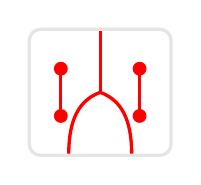
\begin{tikzpicture}[vcenter, scale=0.4]
    \squarecoord
    %
    \path
    (top) edge[string=red] (mid)
    ($(midt)+(1.25,0)$) edge[string=red] ($(midb)+(1.25,0)$)
    ($(midt)-(1.25,0)$) edge[string=red] ($(midb)-(1.25,0)$)
    ;
    \draw[string=red] ($(bot) - (1,0)$)
    to[out=90,in=200] (mid)
    to[out=-20,in=90] ($(bot) + (1,0)$)
    ;
    %
    \node [enddot=red] at ($(midt)+(1.25,0)$) {};
    \node [enddot=red] at ($(midb)+(1.25,0)$) {};
    \node [enddot=red] at ($(midt)-(1.25,0)$) {};
    \node [enddot=red] at ($(midb)-(1.25,0)$) {};
    \draw [rounded corners, draw=black!10, very thick] (-0.25,0) rectangle (4.25,4);
\end{tikzpicture}

\end{document}